\subsection{Technologie- und Methodik-Scouting}
Um auf Grundlage der dargestellten Rahmungen für die Bedarfserkennung und Bereitstellung neuer Fahrumfänge für intelligente Fahrzeuge einen Prototypen zu entwickeln, wird abschließend ein Technologie- und ein Methodik-Scouting durchgeführt werden. Das Kapitel der Arbeitsmethodik spezifiziert Den Zyklus des User-Centered-Designs und stellt dar, weshalb dieser für die Entwicklung des Prototypen die richtige ist. Das anschließende Technologie-Scouting stellt Entwicklungsumbegungen, Frameworks und Programmiersprachen vor, welche in der Entwicklung genutzt werden. 
\subsubsection{Arbeitsmethodik: User-Centered-Design}
Um die Nutzeroberfläche für die Zielgruppen ansprechend zu gestalten, wird bei der Erarbeitung dieser nach den Prinzipien des User-Centered Designs \textit{(UCD)} gehandelt. Ins deutsche übersetzt bedeutet dies "Benutzerzentriertes Design bzw. Benutzerorientierte Gestaltung" eines Produkts. Es beschreibt einen Designprozess bzw. ein Entwicklungsverfahren, "auf welches der Endnutzer (Fahrer) schon von Anfang an Einfluss nimmt" (Vgl. \cite[S.763]{bainbridge2004berkshire}). Der User wird in die Phasen der Entstehung einer Benutzungsschnittstelle integriert was zur Folge hat, “dass der Aufbau, die Inhalte und deren Form sowie das Design des Endproduktes maßgeblich von den Bedürfnissen, Erwartungen und dem Verständnis der User bestimmt wird” (Vgl.\cite{rosenbusch}). Des weiteren kann durch das Einbeziehen von Kunden die Qualität optimiert werden (Vgl. \cite[S. 14]{weisgerber}).\\

"Typisch für einen UCD-Prozess zum Entwerfen von Webanwendungen mit optimaler User Experience sind [jedoch] die Prozessschritte Analyse, Konzeption, Umsetzung/ Design, Evaluierung und Optimierung." (Vgl. \cite{seobility})\\
Im Rahmen der Analyse werden die Anforderungen an das System erstellt und zusammengeführt. Hierzu können Personas erstellt werden (siehe: \ref{personas}) und aus eben diesen können Anforderungen erstellt werden. Die Analyse soll zudem "Usability"\cite{usability-toolkit} Ziele festlegen, anhand welcher in der "Evaluierung und Optimierung" die Güte der Nutzeroberfläche gemessen werden kann \cite{seobility}. Während der Konzeption soll das Verständnis der Benutzer und deren Bedürfnisse hinsichtlich der User Experience auf die Benutzeroberfläche übertragen werden \cite[(ebd.)]{seobility}. Die Konzeption endet mit dem erstellen eines Prototypen. Dieser wird in der Dritten Phase (Design) durch "ein konsistentes, ansprechendes und klares Grafik Design"(Vgl. )\cite{seobility}) erweitert, was Probleme löst und eine Intuitive Bedienung unterstützt. Die Phase der "Evaluierung und Optimierung" wird das Produkt auf Probleme wie Sicherheit oder eine schlechte Bedienbarkeit hin untersucht. Hierdurch werden Mängel entdeckt welche in den nächsten Zyklus der Entwicklung einfließen.\\

Wie hoch der Grad der Usability und der User-Experience ist, lässt sich wie zuvor erwähnt anhand von Personas ableiten. Im Folgenden wird daher erklärt, was Personas sind und es werden eigene Personas für das Projekt erstellt.

\textbf{Personas}\label{personas}\\
Bei Personas handelt es sich nun um fiktive Personen, also hypothetische User, mit individuellen Eigenschaften \cite[]{seibert2008}, welche ebenso eine reale Person haben könnte. Je ähnlicher die Personas also der Zielgruppen des Unternehmens/des Produktes sind, desto effektiver ist die Verwendung dieser.\\
Personas sind nicht nur als potentielle Zielgruppe zu sehen - sie haben zudem die Aufgabe, dass sich das Entwicklerteam in die Position des Nutzers versetzen kann. Dazu werden Personas zunächst nach Kategorien wie "Geschlecht" oder "Alter"  aufgeteilt und anschließend wird jedes Profil mit Merkmalen und Eigenschaften gefüllt. Welche Informationen unter anderem zu Personas hinzugefügt werden, zeigt die folgende Tabelle.
\begin{center}
	\begin{tabular}{| l | l |}
		\hline
		\cellcolor{blue!25}Vor- und Nachname & \cellcolor{blue!25}Geburtsdatum/Alter\\
		\hline
		\cellcolor{blue!25}Foto der Person/Aussehen & \cellcolor{blue!25}Herkunft/Wohnort\\
		\hline
		\cellcolor{blue!25}Sprachkenntnisse & \cellcolor{red!25}Beruf; Berufserfahrung in Jahren\\
		\hline
		\cellcolor{blue!25}Bildung/Ausbildung & \cellcolor{blue!25}Familienstand\\
		\hline
		\cellcolor{red!25}Interessen und Hobbys & \cellcolor{red!25}Fähigkeiten/Behinderungen\\
		\hline
		\cellcolor{green!25}Sicherheitsrisikofaktoren für den Straßenverkehr &\cellcolor{green!25}Abneigungen\\
		\hline
		\cellcolor{green!25}Erfahrungen mit Technik (Meidenkompetenz) & 
		\cellcolor{green!25}Vorlieben \\
		\hline
		\cellcolor{green!25}Fahrerfahrung & \cellcolor{blue!25}Kaufbereitschaft\\
		\hline
		\cellcolor{green!25}Auto; Wenn ja: Besitzverhältnis? & \\
		\hline
	\end{tabular}
\end{center}
Anhand dieser möglichen Informationen werden im folgenden die Personas für dieses Projekt erstellt.
\begin{center}
	\begin{tabular}{| p{0.3\textwidth} | p{0.3\textwidth} | p{0.3\textwidth} |}
		\hline
		\cellcolor{blue!25}Name / Soziographische Daten & \cellcolor{red!25}Hobbys \& Interessen & \cellcolor{green!25}Anwendungsfallbezogenes \\
		\hline
		\vspace{0.3mm}
		\begin{minipage}{.2\textwidth}
			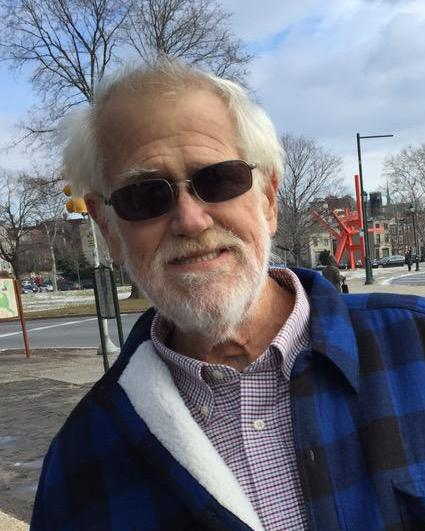
\includegraphics[width=\linewidth]{../pictures/persona1.jpg}
		\end{minipage}
		\begin{itemize}
			\item Dietmar Müller, 68 Jahre (Bild: \cite{persona1})
			\item Loppersum, Ostfriesland
			\item Deutsch 
			\item Gelernter Maurer
			\item Verheiratet, 3 Erwachsene Kinder
		\end{itemize}
		&
		\begin{itemize}
			\item Rentner; Taxiunternehmer(seit 20 Jahren aktiv)
			\item Fischen, Wandern
			\item Handwerklich begabt, Hobbygärtner 
			\item Diabetiker
			\item idR. Minus-Kunde
			\item Geizig
		\end{itemize}	
		& 
		\begin{itemize}
			\item Führerschein seit 47 Jahren
			\item Vertraut Technik nicht
			\item Schlechte Sehkraft
			\item Ängstlicher Autofahrer
			\item Besitzt eigenen Neuwagen
		\end{itemize}
		\\ [0.5ex]
	
		%Persona 2
		\hline
		\vspace{0.3mm}
		\begin{minipage}{.2\textwidth}
			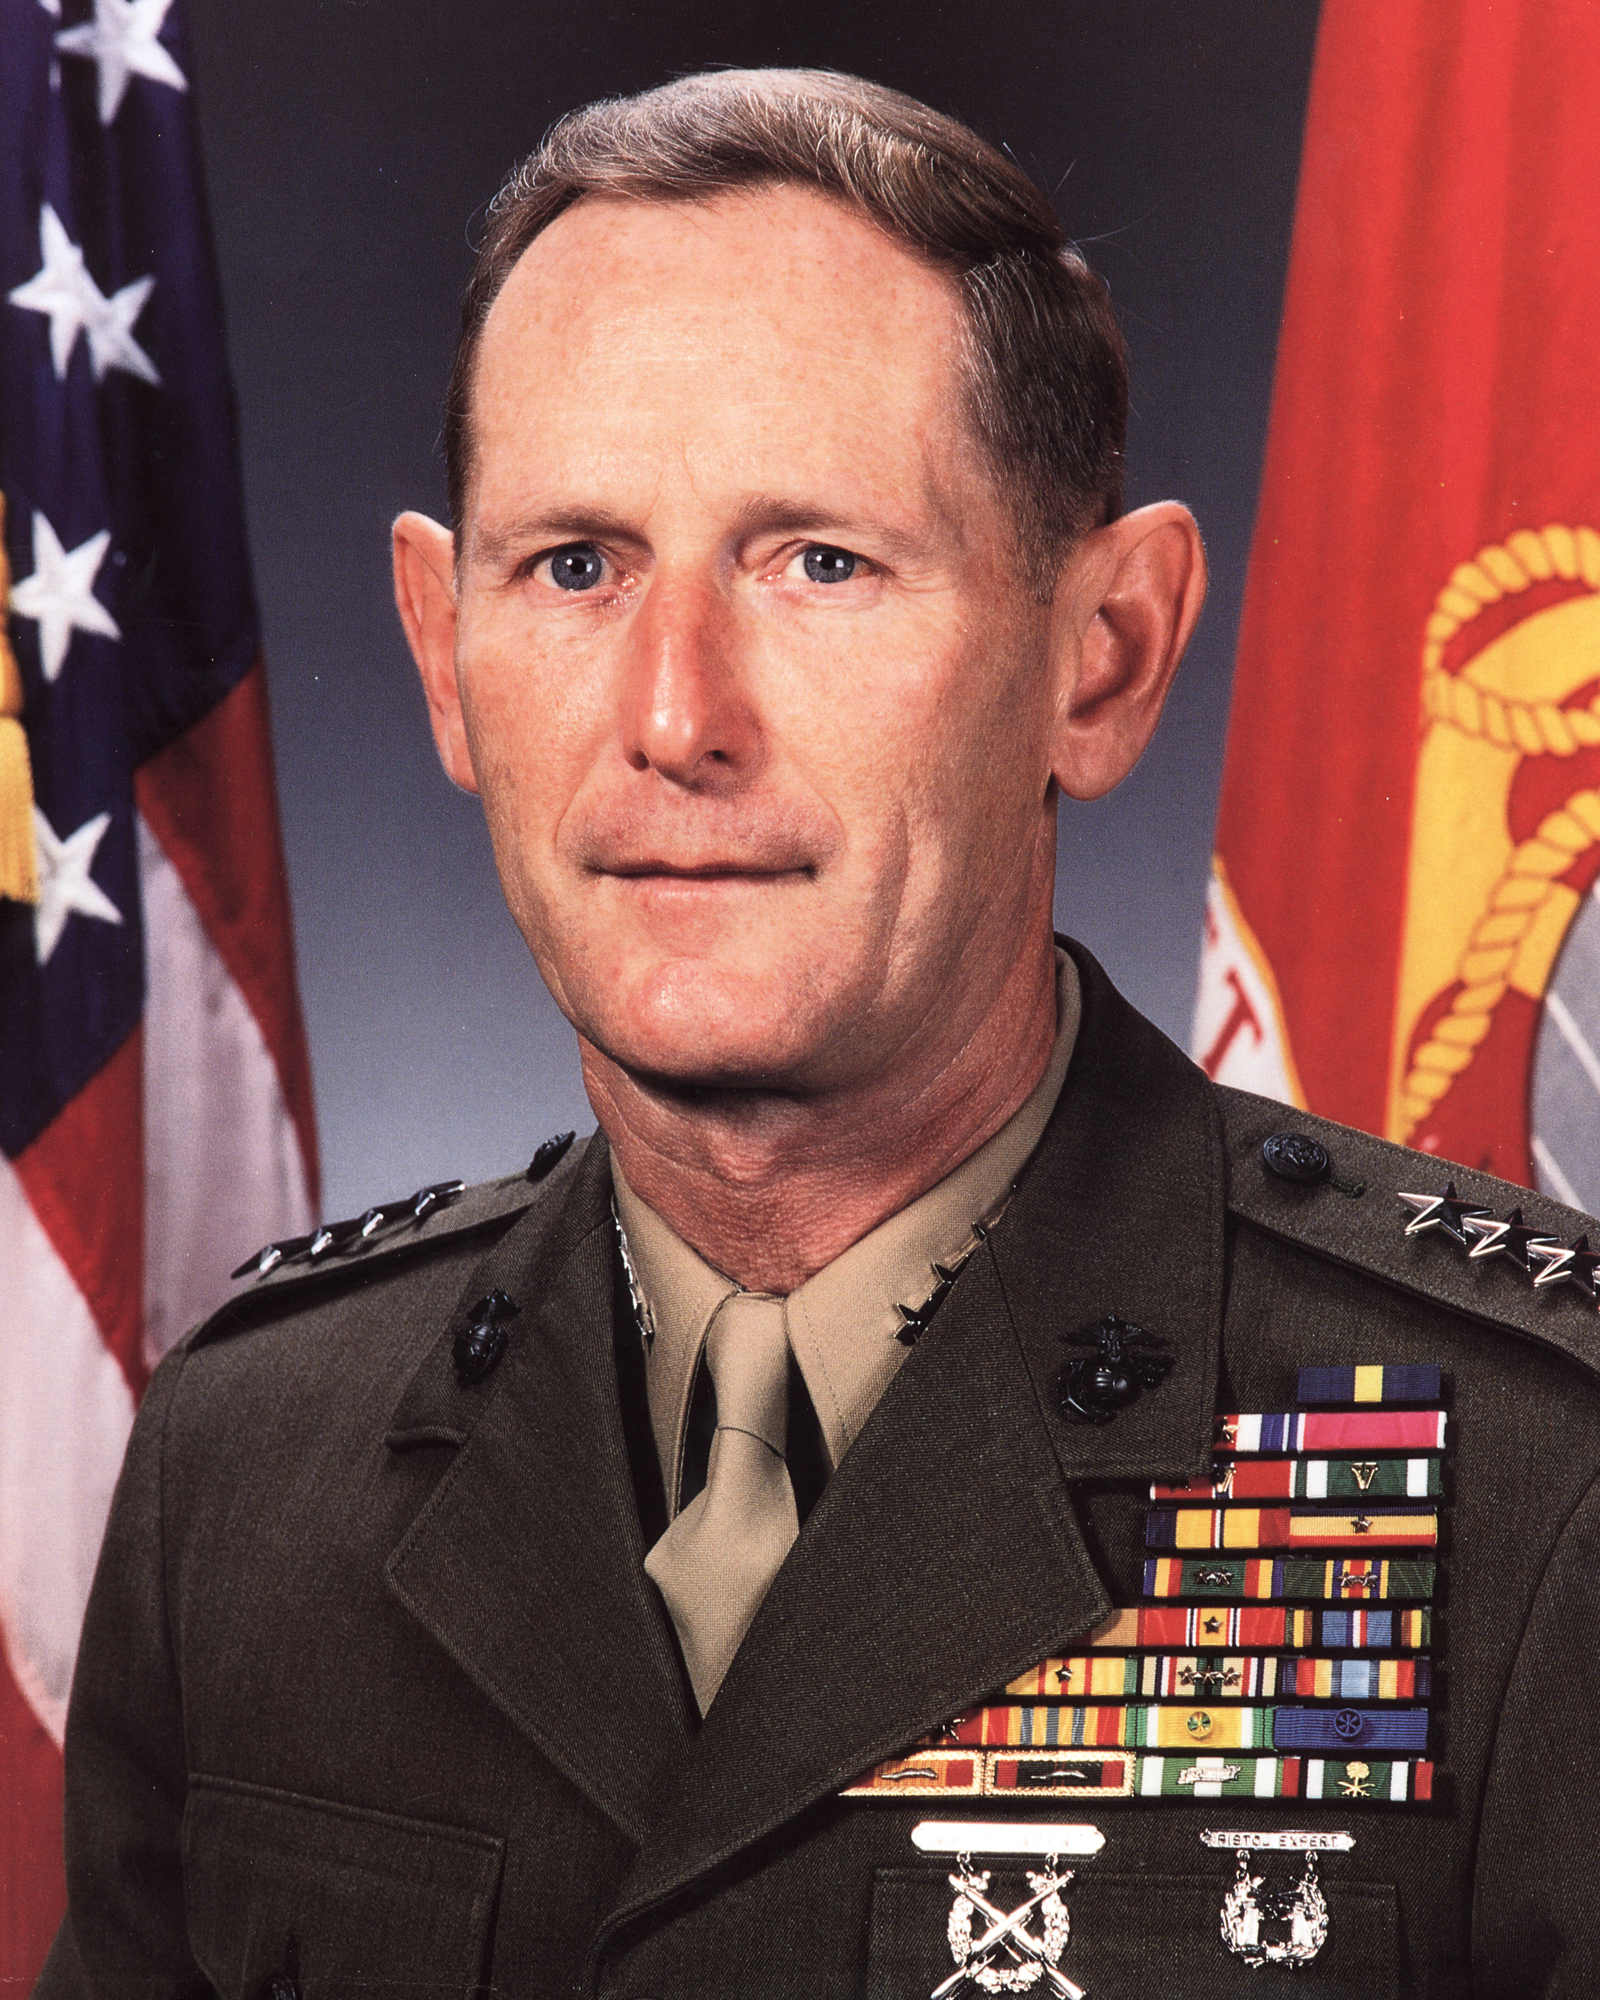
\includegraphics[width=\linewidth]{../pictures/persona2.jpg}
		\end{minipage}
		\begin{itemize}
			\item Jake Schneiders, 52 Jahre (Bild: \cite{persona2})
			\item Washington, USA
			\item Englisch, Russisch(Fließend)
			\item Ausgebildeter Cyberhacker
			\item Geschieden, ein Kind (geteiltes Sorgerecht)
		\end{itemize}
		&
		\begin{itemize}
			\item Leutnant beim Militär
			\item Jagen, Baseball Trainer
			\item Kindersorgerecht unter der Woche
			\item Workaholic
			\item Chancen-Kunde
		\end{itemize}	
		& 
		\begin{itemize}
			\item Führerschein seit 27 Jahren
			\item Vertraut sehr auf Technik
			\item guter, sicherer Autofahrer
			\item Setzt Wert auf gute Bedienbarkeit
			\item Hat gerne die Kontrolle über Systeme
			\item Fährt einen Wagen des Militärs
			\item Arbeitet viel am Laptop
		\end{itemize}
		\\[0.5cm]
		\hline
	\end{tabular}
\end{center}
\begin{center}
	\begin{tabular}{| p{0.3\textwidth} | p{0.3\textwidth} | p{0.3\textwidth} |}	
		\hline
		%Persona 3
		\vspace{0.3mm}
		\begin{minipage}{.2\textwidth}
			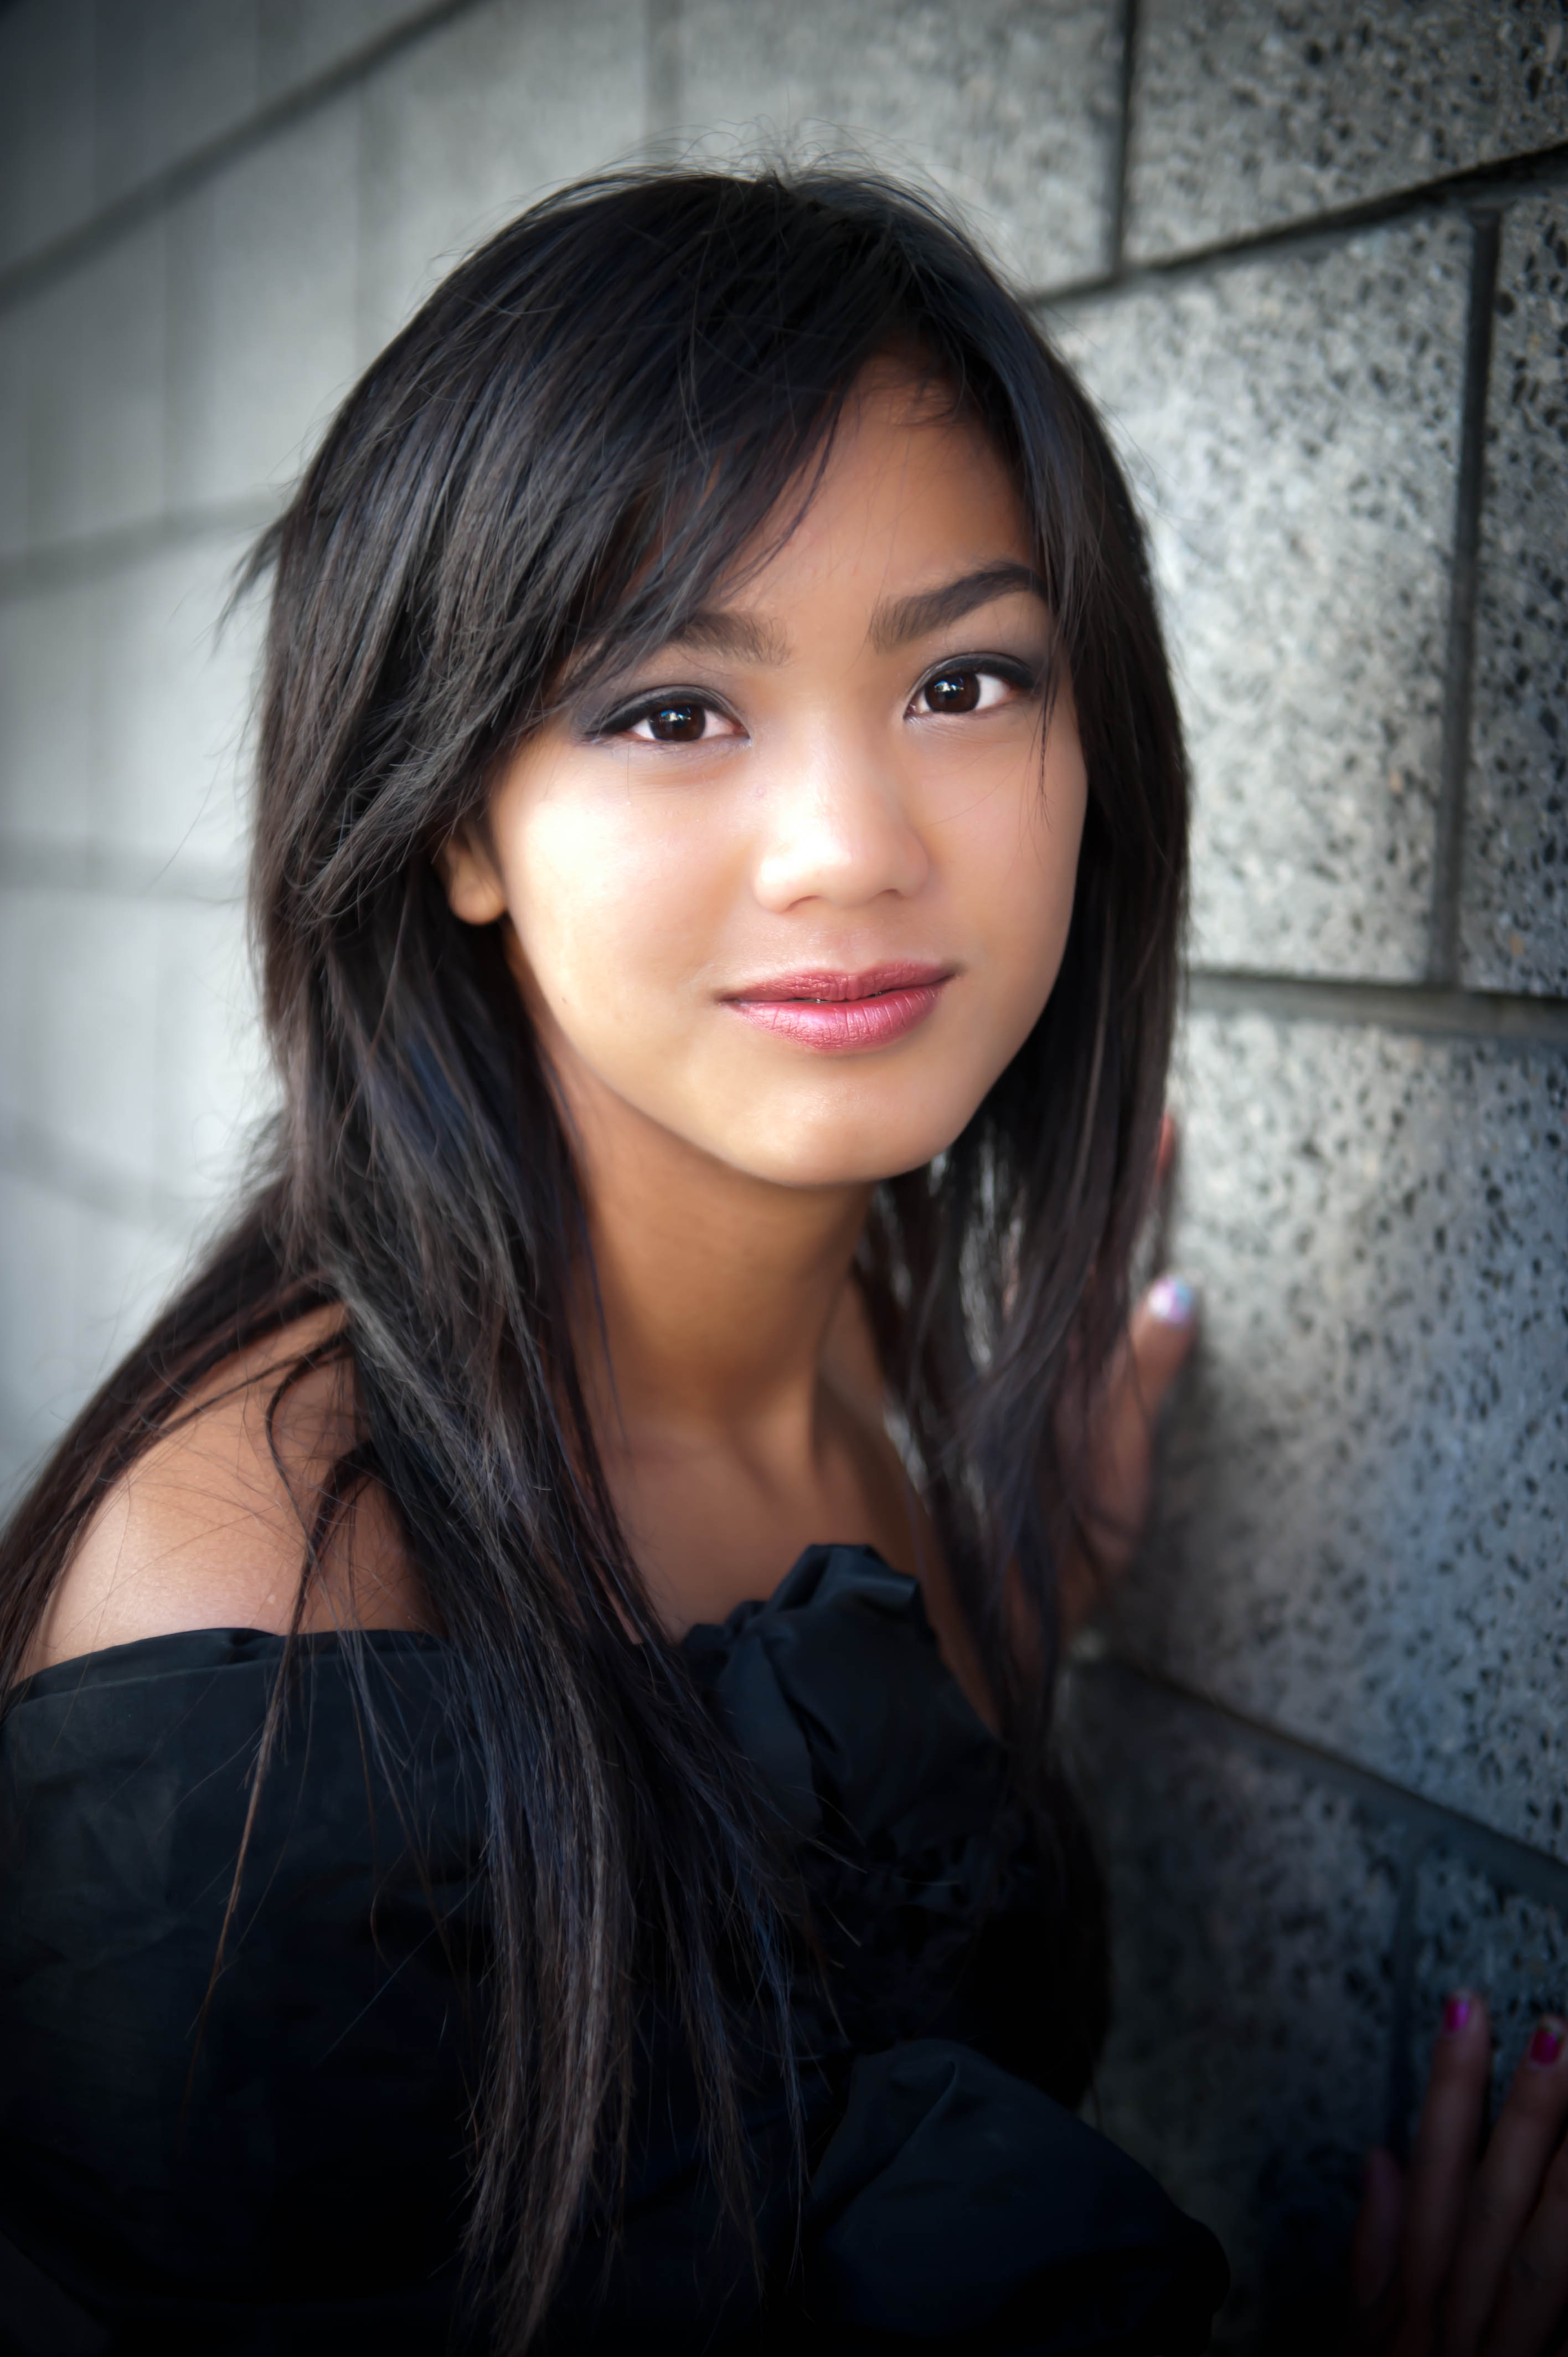
\includegraphics[width=\linewidth]{../pictures/persona3.jpg}
		\end{minipage}
		\begin{itemize}
			\item Chi Nguyen, 24 Jahre (Bild: \cite{persona3})
			\item Rom, Italien
			\item Vietnamesisch, Italienisch(Fließend), Englisch (Fließend)
			\item Studentin (Geschichte)
			\item Single
		\end{itemize}
		&
		\begin{itemize}
			\item Studentin, Stadtführerin in Rom
			\item Joggen, Roadtrips
			\item Influencer
			\item Plus-Kundin
		\end{itemize}	
		& 
		\begin{itemize}
			\item Führerschein seit 2 Jahren
			\item Vertraut sehr auf Technik
			\item unsichere Autofahrerin
			\item Ist mit viel Technik aufgewachsen
			\item Mag es, ihre Apps zu personalisieren
			\item Nimmt Teil an Car-Sharing
		\end{itemize}
		\\
		\hline
	\end{tabular}
\end{center}
Die erstellten Personas werden bei der Erstellung des Prototypen herangezogen um Anforderungen an das System. Jede einzelne ermöglicht es, bestimmte Schwierigkeiten und Herausforderungen genauer darzustellen. So soll Dietmar Müller verdeutlichen, dass ein Kunde möglicherweise doch vom Kauf einer SW überzeugt werden kann, obwohl er idR. ein Minus-Kunde ist. Durch ihn kann auch dargestellt werden, welche weiteren Einflussfaktoren es neben "Stress" o.Ä. gibt, wie bei seine Diabetes Erkrankung.\\
Jake Schneiders soll die Art Person darstellen, welche neugierig ist, die Sicherheit eines System testen möchte und hierzu auch selber in der Lage ist. Durch seine technische Affinität kann er Systeme leicht Verstehen und neue Anforderungen erstellen, die voraussichtlich leicht zu implementieren sind.\\
Chi Nguyen ist eine sehr feminine Studentin welche bereits vielerorts gewohnt hat. Durch ihr Dasein als Influencerin hat sie ein großes Netzwerk an Followern, mit welchen sie ihre Erfahrungen die sie während der Autofahrt sammelt Teilen kann. \\
Da alle Personas in unterschiedlichen Ländern an dem Straßenverkehr teilnehmen, sind die Einflussfaktoren zur Erstellung von Anforderungen sehr vielfältig, was sich positiv auf die Entwicklung auswirken kann.

\subsubsection{Tech-Scouting}
Damit die Entwicklung des Prototypen möglichst simpel sein wird, wird im Folgenden ein Technologie-Scouting durchgeführt. Es soll die Vorteile aufzeigen, welche ausgewählte Entwicklungsumgebungen, Programmiersprachen und Frameworks für die Entwicklung des Prototypen haben.\\

Im Rahmen eines Prototypen für die Erkennung und Bereitstellung neuer Fahrfunktionen für intelligente Fahrzeuge ist es nötig, ein auf der Straße fahrendes Fahrzeug zu Simulieren und dazu eine passende Nutzeroberfläche zu haben, welche als Mensch-Maschine Schnittstelle des Fahrzeugs agiert. Für das Simulieren einer Straßenverkehrssituation wird der OpenSource Simulator \textbf{Carla}\footnote{http://carla.org/} verwendet.
Mit Carla ist es möglich, das eigene Auto zusammen mit anderen Fahrzeugen, Radfahrern, Fußgängern, Hindernissen uvm. auf der Straße darzustellen. Autos können mit Sensoren ausgestattet werden und die aufgenommenen Daten können mittels der Python-API ausgelesen werden. Der Ablauf einer Simulation wird in einem Python-Script spezifiziert. Eine alternative Möglichkeit zur Erstellung einer Simulation ist das einbinden einer OpenSCENARIO-Datei. Es existiert ein Aufsatz auf Carla, wodurch der Simulator den in einer solchen Datei dargestellten Ablauf selber darstellen kann.\\

Für die Erstellung von Python Skripts wird \textbf{"PyCharm"}\footnote{https://www.jetbrains.com/de-de/pycharm/} als Entwicklungsumgebung gewählt. PyCharm ermöglicht eine intuitive und einfache Anbindung an GIT. Da die aus Carla ausgelesenen Daten verarbeitet werden müssen um zu erkennen wann das Auto nicht mehr selbstständig fahren kann, ist die Entwicklung eines Servers notwendig. Neben der Analyse der Simulation soll dieser als Kommunikationszentrale zwischen eben diesem und der Mensch-Maschine-Schnittstelle dienen. Zur Entwicklung des Servers soll das ebenfalls von JetBrains entwickelte \textbf{IntelliJ IDEA}\footnote{https://www.jetbrains.com/de-de/idea/} dienen. Auch IntelliJ bietet eine einfache Anbindung an GIT an - zusätzlich ist die Einbindbarkeit von \textbf{Maven}\footnote{https://maven.apache.org/} zum verwalten von \textit{Dependencies} ein leichtes.\\

Für die Entwicklung der Mensch-Maschine-Schnittstelle wird eine Android App entwickelt - für diese wird \textbf{Android Studio}\footnote{https://developer.android.com/studio} verwendet. Android Studio ermöglicht neben der visuellen auch eine textuelle Bearbeitung von Nutzeroberflächen. Es ist die von Google empfohlene Entwicklungsumgebung und ermöglicht das erstellen von Apps massiv.

Neben Python wird zum entwickeln von Server und MMS hauptsächlich die Programmiersprache Java (Version 1.10) verwendet. Java wurde an der Universität Oldenburg gelehrt und es wird unter anderem zum entwickeln von Android Apps verwendet.